\documentclass[conference]{IEEEtran}

\usepackage{cite}
\usepackage{graphicx}

% correct bad hyphenation here
\hyphenation{op-tical net-works semi-conduc-tor}


\begin{document}
\title{Information Centric Networking}

\author{
	\IEEEauthorblockN{
		Andr\'{e} Diegues - 201206858\\
		F\'{a}bio Teixeira - 201305725
	}

	\IEEEauthorblockA{
		T\'{o}picos Avan\c{c}ados em Redes - CC4037\\
		Departamento de Ciencia de Computadores\\
		Faculdade de Ciencias da Universidade do Porto
	}
}

\maketitle

\begin{abstract}
Hoje em dia, o enorme aumento de tr\'{a}fego de conte\'{u}do e dados entre utilizadores na \textit{Internet} motivou o desenvolvimento de novas ideias de arquitetura de \textit{Internet} que resolvam eficazmente este problema. Uma delas \'{e} a que vamos abordar neste artigo, a \textit{Information Centric Networking} (ICN), que atrav\'{e}s de uma abordagem de pesquisa de informa\c{c}\~{a}o nas redes permite fornecer \`{a} rede um servi\c{c}o mais resiliente a falhas que cumpre as exig\^{e}ncias atuais de distribui\c{c}\~{a}o de conte\'{u}do~\cite{ahlgren}. Vamos abordar o seu funcionamento, as arquiteturas que nasceram desta ideia e estudar se a mudan\c{c}a de arquitetura de \textit{Internet} \'{e} ou n\~{a}o vi\'{a}vel. 
\end{abstract}

\section{Introdu\c{c}\~{a}o}
O paradigma ICN foi baseado numa primeira abordagem de arquitetura \textit{Internet} denominada de TRIAD\cite{triad}, cujo principal objectivo seria facilitar e aliviar cerca de 80\% do tr\'{a}fego de \textit{Internet} que servia apenas para entrega de conte\'{u}do atrav\'{e}s de uma arquitetura \textit{data-centric}, isto \'{e}, um utilizador pede o conte\'{u}do ao servidor em vez de pedir ao \textit{host} que det\'{e}m esse mesmo conte\'{u}do\cite{ahlgren}. A TRIAD define uma nova camada de conte\'{u}do que est\'{a} implementada por \textit{content routers} que encaminham os pedidos aos \textit{content servers} que, de seguida, fornecem o conte\'{u}do~.\\

O ICN procura substituir a arquitetura atual, que \'{e} um modelo de comunica\c{c}\~{a}o \textit{host-to-host}, por uma arquitetura baseada num modelo \textit{data-centric}, tratando o conte\'{u}do como entidade principal na arquitetura das redes. Uma rede com este tipo de arquitetura ganha in\'{u}meras vantagens em rela\c{c}\~{a}o ao modelo \textit{host-to-host}, nomeadamente, na distribui\c{c}\~{a}o de conte\'{u}do, seguran\c{c}a e desenvolvimento de aplica\c{c}\~{o}es\cite{icn}.\\

Existem v\'{a}rias arquiteturas baseadas neste paradigma. Neste artigo vamos abordar algumas destas arquiteturas, nomeadamente as que ganharam mais apoio ao longo do tempo: \\

\begin{itemize}
\item \textit{Data-Object Network Architecture} (DONA)
\item \textit{Publish-Subscribe Internet Technology} (PURSUIT)
\item \textit{Named Data Networking} (NDN) baseada em \textit{Content-Centric Networking} (CCN) 
\end{itemize}



\section{Como funciona o ICN?}

O ICN utiliza o modelo de comunica\c{c}\~{a}o \textit{Publish/Subscribe}. Neste modelo, os emissores, chamados \textit{Publishers}, em vez de enviarem as mensagens diretamente aos recetores espec\'{i}ficos, caracterizam as mensagens publicadas em classes sem conhecimento de quem v\~{a}o ser os subscritores. Por outro lado, os subscritores, chamados de \textit{Subscribers}, demonstram interesse numa ou mais classes e apenas recebem mensagens da(s) classe(s) que subscreveram, tamb\'{e}m sem conhecimento de quem as enviou.\\ %[1] - [https://en.wikipedia.org/wiki/Publish%E2%80%93subscribe_pattern https://en.wikipedia.org/wiki/Publish%E2%80%93subscribe_pattern]

Neste novo paradigma, os dados tornam-se independentes de localiza\c{c}\~{a}o, mem\'{o}ria e meio de transporte, permitindo o armazenamento e replica\c{c}\~{a}o em \textit{cache}. Algo que impulsiona uma melhoria na efici\~{e}ncia, na escalabilidade e na robustez de comunica\c{c}\~{a}o em cen\'{a}rios dif\'{i}ceis. Existem v\'{a}rias abordagens do ICN, todas focadas num novo desenho da arquitetura da Internet atual, com o objetivo de substituir o atual modelo centrado nos \textit{hosts}, para implementar um modelo mais orientado a dados e centrado nos conte\'{u}dos\cite{surveyICN}. A saber:\\



\subsection{DONA}

A resolu\c{c}\~{a}o de nomes no DONA\cite{dona} \'{e} da responsabilidade de uns servidores especializados chamados \textit{Resolution Handlers} (RHs). Existe pelo menos um RH em cada sistema aut\'{o}nomo. Estes \textit{Handlers} est\~{a}o interconectados, formando um servi\c{c}o hier\'{a}rquico de resolu\c{c}\~{a}o de nomes por cima das rela\c{c}\~{o}es interdom\'{i}nio de \textit{routing} existentes, para que seja poss\'{i}vel conciliar resolu\c{c}\~{a}o de nomes com \textit{routing} de informa\c{c}\~{a}o no mesmo sistema. O \textit{Publisher} envia uma mensagem \textit{REGISTER} com o nome do objeto para o seu RH local, que guarda um apontador para o \textit{Publisher}. O RH depois propaga o \textit{REGISTER} para os RHs que tem liga\c{c}\~{a}o, seguindo as rotas estabelecidas, guardando estes RHs o mapeamento entre o nome do objeto e o endere\c{c}o do RH que encaminhou o registo.\\

 Com isto, os \textit{REGISTERs} s\~{a}o replicados nos RHs at\'{e} aos~\textit{tier-1}, e j\'{a} que estes est\~{a}o conectados com os outros todos, o RH que est\'{a} localizado nesse \textit{tier} est\'{a} ciente do que se passa em toda a rede.Para localizar um item, o \textit{Subscriber} envia uma mensagem \textit{FIND} para o RH local, que tamb\'{e}m propaga esta mensagem aos RHs parentes, at\'{e} que \'{e} feito um \textit{match} com o~\textit{tier-1}. Depois seguem-se os apontadores para encontrar o \textit{Publisher}, j\'{a} que o \textit{tier-1} \'{e} conhecedor de toda a estrutura da rede.\\


%'''CCN (Content Centric Networking project. [Online]. Available: http://www.ccnx.org/)'''[[Image:|top]]



\begin{figure}[h]
\centering
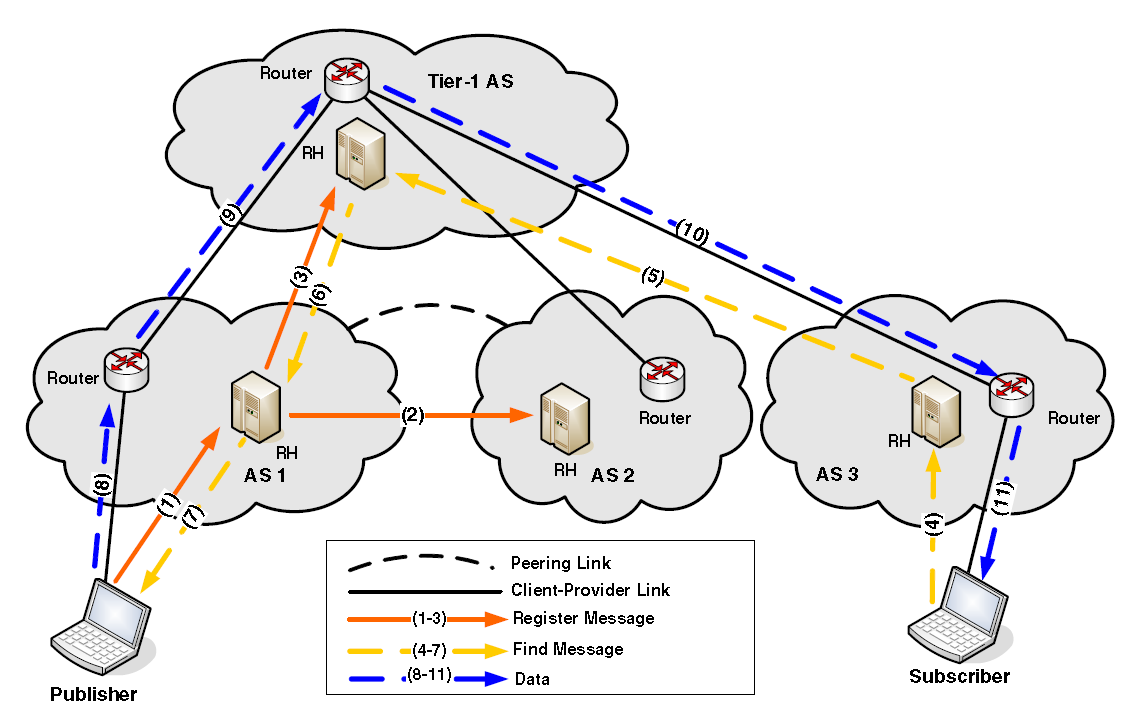
\includegraphics[width=2.5in]{dona}
\caption{DONA implementation.}
\label{dona}
\end{figure}

%'''PURSUIT (FP7 PURSUIT project. [Online]. Available: http://www.fp7-pursuit.eu/PursuitWeb/)'''[[Image:|top]]
\subsection{•}{PURSUIT}

Esta arquitetura substitui completamente a \textit{stack} do protocolo IP por uma \textit{stack} do protocolo \textit{publish-subscribe}. Consiste em tr\^{e}s fun\c{c}\~{o}es distintas: \textit{rendezvous}, \textit{topology management} e \textit{forwarding}.
Quando o \textit{rendezvous} encontra a subscri\c{c}\~{a}o de uma publica\c{c}\~{a}o, direciona a fun\c{c}\~{a}o de gest\~{a}o da topologia para criar uma rota entre o \textit{Publisher} e o \textit{Subscriber}. Esta rota \'{e} usada pela fun\c{c}\~{a}o de encaminhamento para realizar a transfer\^{e}ncia de dados.\\

A resolu\c{c}\~{a}o de nomes no \textit{PURSUIT} \'{e} tratada pela fun\c{c}\~{a}o \textit{rendezvous}, a qual \'{e} implementada por uma cole\c{c}\~{a}o de \textit{Rendezvous Nodes} (RNs), pertencentes \`{a} \textit{Rendezvous Network} (RENE). Quando um \textit{Publisher} quer anunciar um objeto de informa\c{c}\~{a}o, emite uma mensagem \textit{PUBLISH} para o RN local, o qual \'{e} encaminhado por tabelas de \textit{hash} distribu\'{i}das para o RN atribu\'{i}do com o ID do \textit{scope} correspondente. Quando o \textit{Subscriber} emite um \textit{SUBSCRIBE} para o mesmo objeto de informa\c{c}\~{a}o ao seu RN local, \'{e} encaminhado pela tabela de \textit{hash} para o mesmo RN. Depois, o RN informa um n\'{o} da \textit{Topology Management} (TM) para criar uma rota ligando o \textit{Publisher} ao \textit{Subscriber} para entrega de dados. A gest\~{a}o da topologia envia a rota ao \textit{Publisher} numa mensagem \textit{START PUBLISH}, que j\'{a} utiliza a rota para enviar o objeto de informa\c{c}\~{a}o via \textit{Forwarding Nodes} (FNs).\\

\begin{figure}[h]
\centering
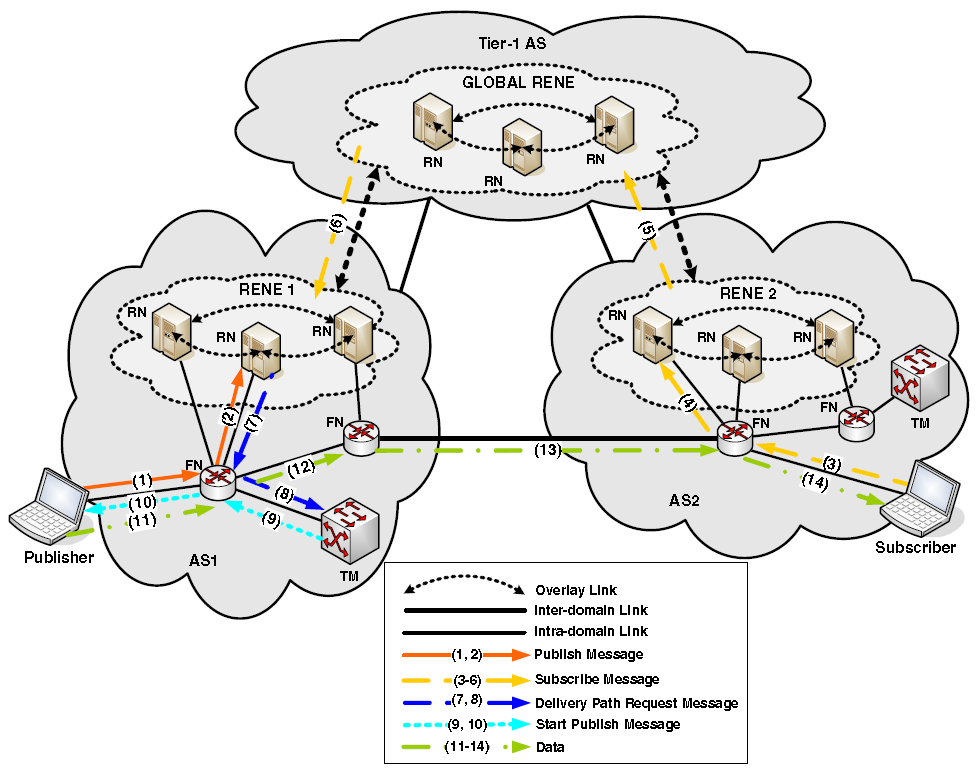
\includegraphics[width=2.5in]{pursuit}
\caption{PURSUIT implementation.}
\label{pursuit}
\end{figure}

% Note that \label must occur AFTER (or within) \caption.
% For figures, \caption should occur after the 
% Note that IEEEtran v1.7 and later has special internal code that
% is designed to preserve the operation of \label within \caption
% even when the captionsoff option is in effect. However, because
% of issues like this, it may be the safest practice to put all your
% \label just after \caption rather than within \caption{}.

%\begin{figure}[!t]
%\centering
%\includegraphics[width=2.5in]{myfigure}
% where an .eps filename suffix will be assumed under latex, 
% and a .pdf suffix will be assumed for pdflatex; or what has been declared
% via \DeclareGraphicsExtensions.
%\caption{Simulation results for the network.}
%\label{fig_sim}
%\end{figure}

%\begin{figure*}[!t]
%\centering
%\subfloat[Case I]{\includegraphics[width=2.5in]{box}%
%\label{fig_first_case}}
%\hfil
%\subfloat[Case II]{\includegraphics[width=2.5in]{box}%
%\label{fig_second_case}}
%\caption{Simulation results for the network.}
%\label{fig_sim}
%\end{figure*}
%
%\begin{table}[!t]
%% increase table row spacing, adjust to taste
%\renewcommand{\arraystretch}{1.3}
% if using array.sty, it might be a good idea to tweak the value of
% \extrarowheight as needed to properly center the text within the cells
%\caption{An Example of a Table}
%\label{table_example}
%\centering
%% Some packages, such as MDW tools, offer better commands for making tables
%% than the plain LaTeX2e tabular which is used here.
%\begin{tabular}{|c||c|}
%\hline
%One & Two\\
%\hline
%Three & Four\\
%\hline
%\end{tabular}
%\end{table}

\subsection{NDN}

Os \textit{Subscribers} emitem mensagens \textit{INTEREST} para pedir informa\c{c}\~{a}o sobre objetos que chegam na forma de dados. As mensagens s\~{a}o encaminhadas por \textit{Content Routers} (CRs), e cada um dos CRs mant\'{e}m tr\^{e}s estruturas de dados: \textit{Forwarding Information Base} (FIB), \textit{Pending Interest Table} (PIT) e \textit{Content Store} (CS). \\

O FIB mapeia informa\c{c}\~{a}o para as interfaces de sa\'{i}da que devem ser usadas para encaminhar as mensagens \textit{INTEREST}. O PIT segue as interfaces de entrada nas quais as mensagens de \textit{INTEREST} chegou. J\'{a} o CS funciona como \textit{cache} local para objetos de informa\c{c}\~{a}o que passaram pelo CR.Quando um \textit{INTEREST} chega, o CR extrai a informa\c{c}\~{a}o do nome e procurar por um objeto nesse CS cujo nome coincida com o prefixo pretendido. Se for bem-sucedido, \'{e} imediatamente enviado atrav\'{e}s da interface de entrada numa mensagem \textit{DATA} e o \textit{INTEREST} \'{e} descartado. Sen\~{a}o, o \textit{router} executa uma procura do prefixo mais longo no seu FIB, para decidir a dire\c{c}\~{a}o do encaminhamento. Se a entrada for encontrada no FIB, o router regista a interface de entrada do \textit{INTEREST} no PIT e empurra o \textit{INTEREST} para o CR indicado pelo FIB.\\

\begin{figure}[h]
\centering
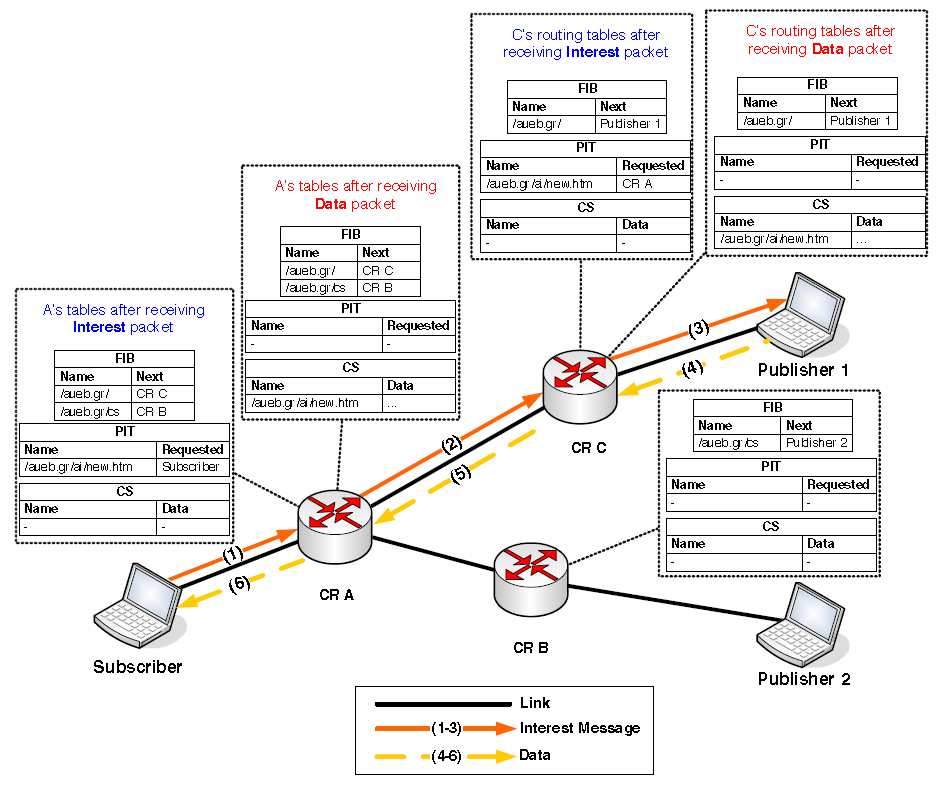
\includegraphics[width=2.5in]{ndn}
\caption{NDN implementation.}
\label{dona}
\end{figure}
\section{Quais os obst\'{a}culos e custos de implementar ICN?}

\subsection{Requisitos}

Uma rede em ICN tem de corresponder a requisitos b\'{a}sicos de modo a ser vi\'{a}vel a sua utiliza\c{c}\~{a}o:


\section{ICN: O futuro da \textit{Internet}}

Os utilizadores est\~{a}o cada vez mais interessados em receber conte\'{u}dos, seja qual for a sua origem, do que ter de aceder a um servidor para receber essa informa\c{c}\~{a}o. E o facto de a \textit{Internet} ainda ser centrada nos \textit{hosts} implica que o utilizador tenha de especificar em cada pedido n\~{a}o s\'{o} a informa\c{c}\~{a}o que deseja receber, como tamb\'{e}m especificar o servidor do qual a informa\c{c}\~{a}o pode ser retirada. Com o ICN isso j\'{a} n\~{a}o acontece\cite{surveyICN}.\\

O pressuposto b\'{a}sico por tr\'{a}s do ICN \'{e} que a informa\c{c}\~{a}o \'{e} nomeada, endere\c{c}ada e encontra o conte\'{u}do independentemente da sua localiza\c{c}\~{a}o. Uma implica\c{c}\~{a}o indireta da implementa\c{c}\~{a}o do ICN \'{e} que a informa\c{c}\~{a}o se torna orientada para o recetor, em contraste com a atual realidade da Internet em que os emissores t\^{e}m controlo total sobre os dados trocados\cite{publishSubscribe}. No ICN s\'{o} s\~{a}o recebidos os dados que o recetor tenha pedido. Depois de ser enviado o pedido, a rede \'{e} respons\'{a}vel por localizar a melhor origem para fornecer a informa\c{c}\~{a}o desejada ao recetor.\\

Quando um elemento da rede receber um pedido por conte\'{u}do, pode ter duas a\c{c}\~{o}es: se estiver em \textit{cache}, responde imediatamente com o conte\'{u}do; se n\~{a}o estiver, faz um pedido aos elementos com os quais tem liga\c{c}\~{a}o e depois guardar em \textit{cache} o conte\'{u}do quando for encontrado\cite{surveyICN}.\\

Nesse sentido, e j\'{a} que os conte\'{u}dos chegam de elementos da rede ao inv\'{e}s da origem, o desenho do ICN tem de garantir a seguran\c{c}a dos conte\'{u}dos, contrariamente \`{a} estrutura atual da Internet que se foca no caminho. Para isso, quem fornece os dados assina um modelo de seguran\c{c}a para que os elementos da rede e os consumidores apenas tenham de verificar essa assinatura para garantir a sua fiabilidade\cite{icnForest}.\\


\section{Conclus\~{a}o}
The conclusion goes here.\\

\IEEEtriggeratref{8}
\IEEEtriggercmd{\enlargethispage{-5in}}

\bibliography{icn}
\bibliographystyle{IEEEtran}

\end{document}


